 \chapter{基于Tagkem的后量子混合模式端到端加密通信协议设计与分析}\label{chap:third}
本章节首先对已有工作进行回顾，并介绍端到端加密协议工作基本流程，再介绍本文的具体研究内容，包括方案设计和方案的安全性分析。
\newcommand{\KDF}{\textsf{KDF}}
\renewcommand{\DH}{\textsf{DH}}
\newcommand{\tg}{\textsf{tag}}
\newcommand{\CT}{\textsf{CT}}
\newcommand{\PK}{\textsf{PK}}
\newcommand{\SK}{\textsf{SK}}
\newcommand{\SSK}{\textsf{SSK}}
\newcommand{\ISK}{\textsf{ISK}}
\newcommand{\RSK}{\textsf{rsk}}
\newcommand{\ESK}{\textsf{ESK}}
\newcommand{\OSK}{\textsf{OSK}}
\newcommand{\PQMSK}{\textsf{PQMSK}}
\newcommand{\IPK}{\textsf{IPK}}
\newcommand{\SPK}{\textsf{SPK}}
\newcommand{\EPK}{\textsf{EPK}}
\newcommand{\OPK}{\textsf{OPK}}
\newcommand{\RPK}{\textsf{rpk}}
\newcommand{\CK}{\textsf{ck}}
\newcommand{\RK}{\textsf{rk}}
\newcommand{\MK}{\textsf{mk}}
\newcommand{\PQMPK}{\textsf{PQMPK}}

\section{基于Tagkem的后量子混合模式端到端加密通信协议设计概述}
端到端加密（End-to-End Encryption, E2EE）作为保障即时通信隐私的核心技术，近年来经历了从理论构建到大规模工业部署的快速发展。其核心目标是在不可信服务器参与的消息传递模型中，确保仅通信双方能够解密消息内容，即使服务提供商也无法访问明文。当前主流 E2EE 协议在安全性、前向保密性（Forward Secrecy）、后向保密性（Post-compromise Security）等方面取得了显著进展，但仍面临效率、可扩展性与抗量子安全等多重挑战。

\textbf{Signal 协议} 是现代 E2EE 的奠基性工作，其提出的 双棘轮机制结合了 X3DH 密钥协商与 KDF 链式派生，实现了强大的会话密钥更新能力，支持异步通信下的前向与后向保密。然而，Signal 依赖于经典 Diffie-Hellman 假设，在量子计算威胁下不再安全。

为应对这一问题，研究者开始探索 \textbf{后量子安全的 E2EE 协议}。\textbf{PQXDH}将 Signal 的 X3DH 扩展为混合密钥交换：结合经典 ECDH 与 NIST 标准化后量子 KEM，在保持兼容性的同时提供量子安全后备。随后，\textbf{PQ3}进一步引入后量子双棘轮结构，能够提供长期后量子安全性。尽管如此，这些方案普遍存在\textit{密钥协商开销大、握手延迟高、密文体积膨胀}等问题，尤其在移动网络或低带宽场景下体验不佳。

针对带宽消耗大的问题，近期研究提出了多种优化技术：
\begin{itemize}
    \item \textbf{Katana} 提出\textit{密文复用机制}\cite{dodis2025triple}，允许多个会话共享同一后量子密文以摊薄计算与带宽成本，但牺牲了会话独立性，可能引入跨会话关联风险；
                                                                    
    \item \textit{纠删码分块技术} 将大体积后量子密文分片并编码，接收方可通过部分分片恢复完整密文，虽提升传输鲁棒性，但密钥复原过程引入显著延迟，影响实时性；
    
    \item \textbf{机会性发送}（Opportunistic Push Protocol, OPP\cite{auerbach2025compare}）利用空闲网络窗口预推送密文，减少用户交互时的等待时间，但其状态管理与调度逻辑设计复杂，工程实现难度高，且难以保证严格的安全边界。
\end{itemize}

综上所述，现有后量子 E2EE 方案在安全性、效率与实用性之间尚未取得理想平衡：要么密钥协商冗余，要么引入额外信任假设或状态复杂性。尤其在群聊、异步消息、设备多端同步等场景中，密钥绑定上下文（如会话 ID、设备标识）的能力显得尤为重要，而传统 KEM 无法天然支持此类语义绑定。

为此，本文提出一种基于 \textbf{标签密钥封装机制}（Tag based Key Encapsulation Mechanism, TagKEM） 的新型 E2EE 架构。该方案通过在密钥派生过程中显式嵌入\textit{上下文标签}（如会话标识符、用户身份、时间戳等），实现密钥与通信语境的强绑定，从而：
\begin{enumerate}
    \item \textbf{避免密文重复封装}：同一公钥可安全地用于多个不同标签的会话，无需为每个会话生成新密文；
    
    \item \textbf{增强密钥隔离性}：不同标签导出的密钥相互独立，防止跨会话密钥推导；
    
    \item \textbf{简化协议状态}：无需维护复杂的会话链或预共享状态，降低实现复杂度；
    
    \item \textbf{兼容后量子 KEM}：可无缝集成 Kyber 等 NIST 标准化方案，兼顾量子安全与工程可行性。
\end{enumerate}
为了实现基于国产后量子密码算法的端到端加密协议自主化演进路径研究，提出基于国密SM系列算法对协议进行改造，具体的，将使用SM2算法承担身份密钥生成、密钥协商和数字签名的角色，使用SM3承担密钥导出函数的角色，使用SM4承担消息对称加密的角色。
下文将详细阐述本方案的设计细节、安全模型与性能分析。

\section{端到端加密协议工作概览}
以Signal App 使用的端到端加密协议为例，为了实现异步通信，发送与接收消息的双方首先需要进行注册，并将对应的预密钥包发布到服务器，初始会话时Alice会向服务器查询Bob的预密钥包信息并下载，然后在本地完成密钥初始化，最后向Bob发送第一条加密信息，Bob接收后完成与Alice的会话初始化。具体的，如下所示：

\textbf{注册阶段}：在协议初始化时，每个用户生成三类密钥对并将其公钥上传至服务器。其中包括长期的身份密钥（Identity Key），用于身份绑定与认证；定期轮换的已签名预密钥（Signed Prekey），由身份私钥签名以确保其真实性；以及一组一次性使用的预密钥（One-time Prekeys），每个仅用于一次会话建立。这些密钥共同构成了异步通信场景下安全握手的基础。

\textbf{会话建立阶段}：当发起方（如 Alice）欲向接收方（如 Bob）发送首条消息时，她从服务器获取 Bob 的上述三类公钥，并生成一个临时的 Diffie–Hellman（DH）密钥对。随后，双方通过扩展的三方或四方 DH 协议（即 X3DH）计算多个共享秘密——包括基于身份密钥、已签名预密钥、一次性预密钥及临时密钥的组合——并将这些共享值拼接后输入密钥派生函数（KDF）。该过程输出一个主密钥，从中派生出初始的根密钥（root key）和发送链密钥（sending chain key），从而完成端到端加密通道的建立。

\textbf{对称棘轮通信阶段}：在会话建立后，通信双方各自维护发送与接收两条密钥链。每发送或接收一条消息，发送方或接收方即利用当前链密钥通过 KDF 派生出一个唯一的消息密钥用于加密或解密，并同步更新链密钥以供下一次使用。该对称棘轮机制确保了前向安全：即使某时刻的链密钥被泄露，历史消息仍因对应消息密钥已被丢弃而无法被解密。

\begin{figure}[htbp]
  \centering
  
    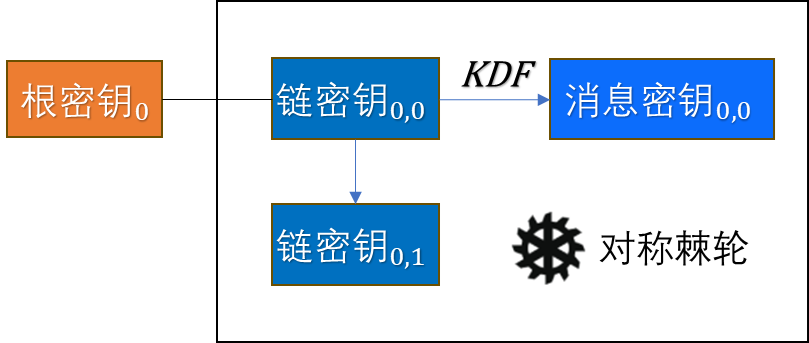
\includegraphics[width=0.4\linewidth]{Img/对称棘轮.png} 
    \caption{对称棘轮示例}
    \label{fig:perf-comparison}
  
  \label{fig:performance}
\end{figure}

\textbf{非对称棘轮更新阶段}：当一方收到包含新棘轮公钥的消息时，触发非对称棘轮过程。接收方利用该新公钥与其本地存储的一个或多个棘轮私钥执行 DH 计算，将所得共享秘密与当前根密钥一同输入 KDF，从而派生出新的根密钥及全新的发送/接收链。此机制实现了后向安全（Post-Compromise Security）：即便攻击者曾完全攻破设备并获取所有当前密钥，只要后续一次 DH 交换未被破坏，通信即可“自愈”，恢复对未来消息的保密性。
\begin{figure}[htbp]
  \centering
  
    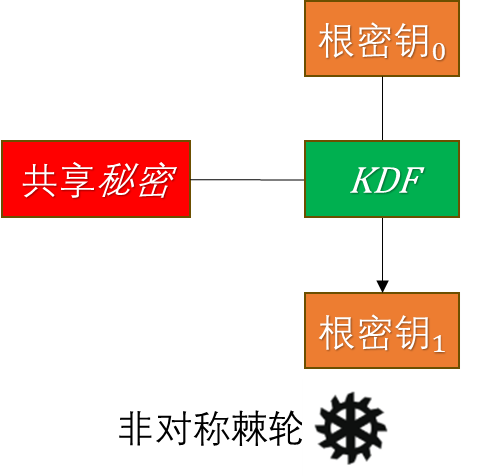
\includegraphics[width=0.3\linewidth]{Img/非对称.png} 
    \caption{非对称棘轮示例}
    \label{fig:perf-comparison}
  
  \label{fig:performance}
\end{figure}

\section{方案设计}
接下去介绍本文方案的具体设计。
本文 协议是一种端到端加密消息协议，旨在支持两台设备之间在长期会话中安全交换数据，并提供经典密码学与后量子密码学相结合的混合安全保证。

本文协议的主要安全目标如下：

\begin{itemize}
    \item \textbf{机密性}：确保发送方与接收方之间的应用层数据对敌手保密，包括抵御具备未来量子计算能力的攻击者所实施的“现在存储、日后解密”（store now, decrypt later）攻击。
    
    \item \textbf{认证性}：允许接收方可靠地识别消息的发送方身份。
    
    \item \textbf{会话密钥的前向安全性}：若某参与方的状态（包括其长期密钥）在某一时刻被泄露，则此前传输的密文无法被解密（前提是对应消息已在被攻陷设备上删除）。
    
    \item \textbf{逐消息前向安全性}：前向安全性应以单条消息为粒度实现。
    
    \item \textbf{会话密钥的后向安全性}：若某设备在某一时刻被攻陷，但随后通过安全措施恢复（例如检测并清除了恶意软件），则设备恢复之后传输的密文不应能被解密。  
    后泄露安全性应以每次往返通信为单位提供；若因后量子密文体积较大导致带宽开销过高，可将后量子后泄露安全性分摊至多个往返通信周期中实现。
    
    \item \textbf{抗重放攻击}：协议应能检测并丢弃重放的消息。
    
    \item \textbf{异步通信支持}：消息可通过中继服务器在任意时间发送与接收，无需发送方与接收方同时在线交互。
\end{itemize}


\subsection{tagkem设计}
为了能够优化通信时带宽的消耗，本文基于后量子密钥封装机制构造一个带标签的密钥封装机制（tag-KEM），记为 $\tkem$。该设计参考 \cite{abe2005tag}，适用于后量子端到端加密协议中的根密钥协商与会话密钥更新阶段。
TKEM 的核心思想是：在密钥派生过程中引入一个公开的标签 $tag$，使得最终输出的共享密钥不仅依赖于公私钥对，还显式绑定于特定通信上下文（如用户身份、会话标识、时间戳等）。
尽管 $tag$ 是公开可访问的，该机制仍能有效防止密钥复用、重放攻击和跨上下文密钥混淆。

我们采用基于KEM和哈希的方法实现该构造，其安全性依赖于底层 KEM 的 IND-CCA2 安全性、哈希函数的抗碰撞性以及密钥派生函数的伪随机性。                

具体算法如下所示：


\begin{algorithm}[H]
\caption{ $ \mathsf{TKEM}.\mathsf{Enc}(PK, \mathsf{tag}) $ }
\label{alg:tkem_enc}
\begin{algorithmic}[1]


\State  $ m \gets \{0,1\}^{256} $ 
\State  $ (k^*, r) \gets G(H(\mathsf{PQMPK}, m, \mathsf{tag})) $ 
\State  $ ct \gets \mathsf{PKE}.\mathsf{Enc}(\mathsf{PQMPK}, m; r) $ 
\State  $ k_{\text{out}} \gets H(k^*, H(ct)) $ 
\State \Return  $ (ct, ss)) $ 
\end{algorithmic}
\end{algorithm}

\begin{algorithm}[H]
\caption{ $ \mathsf{TKEM}.\mathsf{Dec}(SK, ct, \mathsf{tag}) $ }
\label{alg:tkem_dec}
\begin{algorithmic}[1]


\State  $ m' \gets \mathsf{PKE}.\mathsf{Dec}(\mathsf{PQMSK}, ct) $ 
\If{ $ m' = \bot $ }
    \State \Return  $ \bot $ 
\EndIf
\State  $ (k^{*\prime}, r') \gets G(H(\mathsf{PQMPK}, m', \mathsf{tag})) $ 
\State  $ ct' \gets \mathsf{PKE}.\mathsf{Enc}(\mathsf{PQMPK}, m'; r') $ 
\If{ $ ct' = ct $ }
    \State  $ ss \gets H(k^{*\prime}, H(ct)) $  
\Else
    \State  $ ss \gets H(z, H(ct)) $   \Comment{Error path}
    
\EndIf
\State \Return  $ ss $ 
\end{algorithmic}
\end{algorithm}




\subsection{tagkem安全性分析}
接下去我们对tagkem的安全性进行分析，我们定义本文提出的 TKEM 方案在选择密文攻击下具有不可区分性（IND-CCA2）。在该构造中，后量子（PQ）私钥 $sk$ 在长寿命会话中保持静态，而标签 $\tau$ 随每次消息发送通过非对称棘轮更新（注入了新鲜的经典 ECDH 公钥材料）。

\begin{theorem}
假设 $\mathcal{K}$ 是一个满足 IND-CCA2 安全性的封装机制（KEM），且密码学哈希函数 $H$ 被建模为随机预言机（Random Oracle），则该 TKEM 构造在“静态私钥-动态标签”模型下满足 IND-CCA2 安全性。
\end{theorem}

\begin{proof}
我们通过一系列博弈（Games）来限制量子对手 $\mathcal{A}$ 攻破 TKEM 的优势。令 $Adv_{\mathcal{A}}^{G_i}$ 表示 $\mathcal{A}$ 在博弈 $G_i$ 中的优势。

\paragraph{Game 0.} 这是标准的 IND-CCA2 安全实验。挑战者生成 $(pk, sk) \leftarrow \mathsf{Gen}(1^\lambda)$。对手 $\mathcal{A}$ 获得 $pk$ 并可访问解封装谕示器 $\mathcal{O}_{Decaps}(c, \tau)$。
\begin{itemize}
    \item \textbf{挑战阶段：} $\mathcal{A}$ 选择目标标签 $\tau^*$。挑战者计算 $(c^*, K_0^*) \leftarrow \mathsf{Encaps}(pk, \tau^*)$ 并随机选择 $K_1^*$。抛硬币 $b \in \{0, 1\}$，将 $(c^*, K_b^*)$ 返回给 $\mathcal{A}$。
    \item \textbf{限制条件：} 挑战后，$\mathcal{A}$ 禁止查询 $\mathcal{O}_{Decaps}(c^*, \tau^*)$。
\end{itemize}



\paragraph{Game 1 (标签唯一性).} 在此博弈中，我们假设棘轮机制生成的标签 $\tau$ 在会话中是唯一的。由于 $\tau$ 包含了新鲜的 ECDH 公钥，在随机预言机模型下，标签碰撞 $\tau_i = \tau^*$ 的概率 $\leq q^2 / 2^{|\tau|}$（$q$ 为会话数），该概率可忽略不计。

\paragraph{Game 2 (预言机挑战).} 挑战者在不使用 $sk$ 的情况下仿真 $\mathcal{O}_{Decaps}(c, \tau)$：
\begin{itemize}
    \item 对于任何 $\tau \neq \tau^*$ 的查询，利用随机预言机 $H$ 的域隔离（Domain Separation）属性：即便内部 KEM 秘密 $ss$ 相同，由于输入标签不同，输出密钥 $K = H(ss, \tau)$ 在计算上独立于挑战密钥 $K^* = H(ss, \tau^*)$。
    \item 若 $\mathcal{A}$ 能识别此变化，则意味着 $H$ 发生了碰撞或违反了随机预言机假设。
\end{itemize}
$|Pr[G_2] - Pr[G_1]| \leq \epsilon_{ROM}$。

\paragraph{Game 3 (归约至底层 KEM 安全性).} 我们将挑战密文内的 KEM 共享秘密 $ss^*$ 替换为真正的随机值 $ss_{rand}$。
\begin{itemize}
    \item 如果 $\mathcal{A}$ 能区分 Game 3 和 Game 2，则可以构造一个算法 $\mathcal{B}$ 攻破底层 PQ-KEM 的 IND-CCA2 安全性。
    \item $\mathcal{B}$ 将其自身的 KEM 挑战 $(c_{kem}^*, ss_{kem}^*)$ 嵌入到 TKEM 的挑战中。
\end{itemize}
$|Pr[G_3] - Pr[G_2]| \leq Adv_{\mathcal{K}}^{IND-CCA2}(\mathcal{B})$。



\paragraph{Game 4 (密钥独立性).} 在 Game 3 中，挑战密钥 $K_0^*$ 现在是 $H(ss_{rand}, \tau^*)$。由于 $ss_{rand}$ 是随机生成的且未在别处使用，在对手 $\mathcal{A}$ 的视角下，$K_0^*$ 与随机密钥 $K_1^*$ 在统计上不可区分。
因此，$Pr[G_4] = 1/2$。

\paragraph{结论.}
综上所述，对手的优势上限为：
\begin{equation}
    Adv_{TagKEM}^{IND-CCA2}(\mathcal{A}) \leq Adv_{\mathcal{K}}^{IND-CCA2}(\mathcal{B}) + \frac{q_H}{2^\lambda} + \text{negl}(\lambda)
\end{equation}
证明完毕。即使 $sk$ 被重复使用，只要底层 KEM 满足 CCA2 安全且标签与会话强绑定，会话密钥对量子对手依然是安全的。
\end{proof}


\subsection{多阶段密钥交换协议设计}

设 $P$ 为一个参与方。我们将 $P$ 的第 $p$ 次会话记为 $\pi_{P,p}$。  
一次会话指某参与方执行协议的一次完整运行，对应于双方在一条长期聊天（中各自维护的状态。 在 Alice 与 Bob 之间的长期聊天中，共存在两个会话：Alice 端的一个会话和 Bob 端的一个会话。

每个会话内部包含多个阶段，每个阶段会建立一个共享密钥。在 Signal 及 PQ3 协议中，这些阶段可被组织为一棵阶段树：

\begin{itemize}
    \item 树的主干（trunk）由初始握手阶段及后续通过非对称棘轮（生成的阶段构成，依次记为 $[\mathsf{asym}_0], [\mathsf{asym}_1], [\mathsf{asym}_2], \dots$。
    
    \item 从每个主干阶段 $[\mathsf{asym}_j]$ 分支出两条链：
    \begin{itemize}
        \item 接收链（incoming chain）$\mathsf{in}[j]$，用于生成解密密钥，
        \item 发送链（outgoing chain）$\mathsf{out}[j]$，用于生成加密密钥。
    \end{itemize}
    这两条链通过对称棘轮推进，其上的阶段分别记为 $[\mathsf{in}_{j,0}], [\mathsf{in}_{j,1}], \dots$ 和 $[\mathsf{out}_{j,\ell}], \dots$。
    

\end{itemize}
隐式地，每条链均维护其当前长度，记为 $\bigl|[\mathsf{chain}]\bigr|$。
\begin{definition}[参与方和会话状态定义]
每个参与方 $P \in [n_p]$ 拥有：
\begin{itemize}
  \item 长期身份密钥对 $(IPK_P, ISK_P)$；
  \item 后量子 KEM 的长期密钥对 $(PQMPK_P, PQMSK_P)$，由 $\mathsf{Aigis.KGen}()$ 生成，其中私钥 $PQMSK_P$ 是不可泄露的，不允许通过任何攻击者查询（如 $\mathsf{Corrupt}$）被获得。
我们使用 $\pi_P^i$ 表示参与方 $P$ 的第 $i$ 个会话状态，每个 $\pi_P^i$ 维护如下字段：
\begin{align*}
  &\mathsf{oid} \in [n_p] && \text{：会话所属者 ID} \\
  &\mathsf{pid} \in [n_p] \cup \{\bot\} && \text{：对端 ID} \\
  &\mathsf{role} \in \{\mathsf{init}, \mathsf{resp}\} && \text{：角色（发起者/响应者）} \\
  &\mathsf{status\_exec}[s] \in \{\bot, \mathsf{running}, \mathsf{accepted}, \mathsf{rejected}\} && \text{：会话阶段 } s \text{ 执行状态} \\
  &\mathsf{st}[s] && \text{：上一个会话状态值，包括根密钥等} \\
  &\mathsf{sid}[s] \in \{0,1\}^* && \text{：会话标识符} \\
  &K[s] \in \mathcal{k}_{\mathsf{KE}} \cup \{\bot\} && \text{：派生的会话密钥} \\
  &\mathsf{rnd}[s] && \text{：用于非对称棘轮更新的随机数} \\
  &\mathsf{tag}[s] && \text{：KEM 中使用的标签 } tag \\
  &t[s] \in \{\mathsf{init}, \mathsf{ratchet\_asy}, \mathsf{ratchet\_sym}\} && \text{：会话阶段 } s \text{ 类型} \\
  &\mathsf{ct} && \text{：KEM 密文 ciphertext}
\end{align*}
\end{itemize}
\end{definition}


\begin{definition}[多阶段密钥交换协议]
一个多阶段密钥交换协议 $\Pi$ 是多个算法的组合，具体如下：

\begin{itemize}
  \item $\mathsf{KeyGen}() \rightarrow (LtPK, LtSK)$：概率长期密钥生成算法，输出一个长期公钥/秘密密钥对 $(LtPK, LtSK)$，对所有密钥生成的一个抽象定义，包括长期椭圆曲线身份密钥和后量子密钥。

  \item $\mathsf{PKBGen}(LtSK) \rightarrow (preepk_{P,i},preesk_{P,i},pqpk_{P},pqsk_{P},σ)$：概率性的预密钥包生成算法，它以长期密钥 $LtSK$ 作为输入，输出签名椭圆曲线公钥/密钥对 $(SSpk, SSsk)$、长期后量子密钥对和签名。

  \item $\mathsf{SessionStart}_S (\pi_{P,p}, IPK_R, PKB_{R,i})  \rightarrow (\pi'_{P,p},msg) $：一种概率型发送方会话启动算法，其输入包括：会话状态 π、接收方的身份公钥 $IPK_R$、预密钥包 $PKB_{R,i}$ ，该算法会更新会话状态为 $\pi'$，同时生成一条发送给对端的消息，这个消息包含一个椭圆曲线公钥、标签、后量子封装密文和消息签名。

  \begin{algorithm}[H]
    \caption{$\mathsf{SessionStart_S}(\pi_{S,s}, \mathsf{IPK}_{R}, \mathsf{PKB_{R,i}})$}
    \label{alg:asym_ratchet}
    \begin{algorithmic}[1]
        \State //验证预密钥包
        \State $S.ver(IPK_R,PKB_{R,i},\sigma)$
        \State $(\mathsf{rpk}_{S,s,1}, \mathsf{rsk}_{S,s,1}) \gets \mathsf{SM2}.\mathsf{KeyGen}()$ 
        \State $\mathsf{ecss}_1 \gets \mathsf{DH}(\mathsf{rsk}_{S,s,1}, \mathsf{preepk}_{R,i})$
        \State $(\mathsf{pqss}_1, \mathsf{pqct_1}) \gets \mathsf{TKEM}.\mathsf{Enc}(\mathsf{pqsk}_{S,s},\mathsf{tag}_{S,s,1})$
        \State $(\mathsf{rk}, \mathsf{ck}) \gets \mathsf{HKDF}(\mathsf{ecss}_1, \mathsf{pqss}_1)$
        \State $\pi_{S,s}.\mathsf{rk}[\mathsf{asmy_0}] \gets \mathsf{rk}$ \Comment{设置第一个根密钥}
        \State $\pi_{S,s}.\mathsf{ck}[\mathsf{out_{0,0}}] \gets \mathsf{ck}$ \Comment{初始化发送链}
        
        
        \State \textbf{Save} $\mathsf{rsk}_{S,s,1}$ \Comment{保存会话状态}
    \end{algorithmic}
    \end{algorithm}

  \item $\mathsf{SessionStart}_R  (\pi_{R,r}, IPK_S, PKB_{R,i}, msg)\rightarrow (\pi'_{R,p},msg) $：一种概率型接收方会话启动算法，其输入包括：会话状态 $\pi$、发送方的身份公钥 $IPK_S$、预密钥包 $PKB_{R,i}$ ，该算法会更新会话状态为 $\pi'$，同时生成一条发送给对端的消息，这个消息包含一个椭圆曲线公钥、标签、后量子封装密文和消息签名。

    \begin{algorithm}[H]
    \caption{$\mathsf{SessionStart_R}(\pi_{R,r}, IPK_S, PKB_{R,i}, msg,\sigma)$}
    \label{alg:asym_ratchet}
    \begin{algorithmic}[1]
        \State //验证msg的数字签名
        \State $S.Ver(IPK_S, msg, \sigma)$
        \State //根据预密钥包的公钥得到对应私钥
        \State $get preesk_{R,i} with PKB_{R,i}$
        \State //计算椭圆曲线共享秘密和后量子共享秘密，并恢复密钥

        \State $\mathsf{ecss}_1 \gets \mathsf{DH}(\mathsf{preesk}_{R,i}, \mathsf{rpk}_{S,s,1})$
        \State $\mathsf{pqss}_1 \gets \mathsf{TKEM}.\mathsf{Dec}(\mathsf{pqsk}_{S}, \mathsf{pqct}_{S,s,1}, \mathsf{tag}_{S,s,1})$
        \State $(\mathsf{rk}, \mathsf{ck}) \gets \mathsf{HKDF}(\mathsf{ecss}_1, \mathsf{pqss}_1)$
        \State $\pi_{P,p}.\mathsf{ck}[\mathsf{in_{0, 0}}] \gets \mathsf{ck}$ \Comment{初始化接收链}

        \State $(\mathsf{rpk}_{R,r,2}, \mathsf{rsk}_{S,s,2}) \gets \mathsf{SM2}.\mathsf{KeyGen}()$
        \State $\mathsf{ecss}_{2} \gets \mathsf{DH}(\mathsf{rpk}_{S,s,1}, \mathsf{rsk}_{R,r,2})$ 
        \State $(\mathsf{pqct}_{R,r,2}, \mathsf{pqss}_{1}) \gets \mathsf{TKEM}.\mathsf{Enc}(\mathsf{pqpk}_{S}, \mathsf{tag}_{R,r,2})$
        \State $(\mathsf{rk'}, \mathsf{ck'}) \gets \mathsf{HKDF}(\mathsf{rk}, \mathsf{ecss}_{2}, \mathsf{pqss}_{2})$ \Comment{非对称棘轮更新，更新根密钥}
        \State $\pi_{R, r}.\mathsf{rk}[\mathsf{asmy_1}] \gets \mathsf{rk'}$ \Comment{设置第一个根密钥}
        \State $\pi_{R,r}.\mathsf{ck}[\mathsf{out_{1, 0}}] \gets \mathsf{ck'}$ \Comment{初始化发送链}
        \State \textbf{Save} $\mathsf{rsk}_{R,r,2}$ \Comment{保存会话状态}
    \end{algorithmic}
    \end{algorithm}
    
    
 



  \item $\mathsf{AsymRatchet}(\pi_{P,p}, \mathsf{rpk}_{P',p',j+1}, \mathsf{pqct}_{P',p',j}, \mathsf{tag}_{P',p',j+1}), \sigma) $：在收到来自其对等方的消息，该消息包含可用于创建新的非对称轮换阶段的短暂公钥后，会话 $\pi_{P,p}$ 中的 参与方$P$ 通过算法\ref{alg:asym_ratchet11}所示的方式，将非对称棘轮推进。当 AsymRatchet 结束时，就完成了 $[asym_j]$ 和 $[asym_{j+1}]$ 的根密钥的更新，以及更新接收链和发送链的链密钥。
    \begin{algorithm}[H]
    \caption{$\mathsf{AsymRatchet}(\pi_{P,p},\mathsf{rpk}_{P',p',j+1}, \mathsf{pqct}_{P',p',j}, \mathsf{tag}_{P',p',j+1}), \sigma$}
    \label{alg:asym_ratchet11}
    \begin{algorithmic}[1]
        \State //验证签名
        \State $j \gets |\pi_{P,p}.\mathsf{asym}|$ \Comment{获取当前状态最新索引}
        \State //恢复密钥
        \State $\mathsf{ecss}_j \gets \mathsf{DH}(\mathsf{rsk}_{P,p,j}, \mathsf{rpk}_{P',p',j+1})$
        \State $\mathsf{pqss}_j \gets \mathsf{TKEM}.\mathsf{Dec}(\mathsf{pqsk}_{P,p}, \mathsf{pqct}_{P',p',j}, \mathsf{tag}_{P',p',j})$
        \State $(\mathsf{rk}, \mathsf{ck}) \gets \mathsf{HKDF}(\mathsf{ecss}_j, \mathsf{pqss}_j)$
        \State $\pi_{P,p}.\mathsf{ck}[\mathsf{in_{j, 0}}] \gets \mathsf{ck}$ \Comment{出发非对称棘轮，初始化一条新的接收链}
        
        \State //生成新的密钥材料用于更新根密钥和链密钥
        \State $(\mathsf{rpk}_{P,p,j+2}, \mathsf{rsk}_{P,p,j+2}) \gets \mathsf{SM2}.\mathsf{KeyGen}()$
        \State $\mathsf{ecss}_{j+1} \gets \mathsf{DH}(\mathsf{rpk}_{P',p',j+1}, \mathsf{rsk}_{P,p,j+2})$ 
        \State $(\mathsf{pqct}_{P,p,j+2}, \mathsf{pqss}_{j+1}) \gets \mathsf{TKEM}.\mathsf{Enc}(\mathsf{pqpk}_{P',p'}, \mathsf{tag}_{P,p,j+2})$
        \State $(\mathsf{rk}_{P,p,j+2}, \mathsf{ck}_{P,j+2}) \gets \mathsf{HKDF}(\mathsf{rk}, \mathsf{ecss}_{j+1}, \mathsf{pqss}_{j+1})$
        \State $\pi_{P, p}.\mathsf{rk}[\mathsf{asmy_{j+1}}] \gets \mathsf{rk'}$ \Comment{更新根密钥}
        \State $\pi_{P,p}.\mathsf{ck}[\mathsf{out}, j+1, 0] \gets \mathsf{ck}_{P,p,j+2}$ \Comment{更新发送链}
        \State \textbf{Save} $\mathsf{rsk}_{P,p,j+2}$ \Comment{持久化状态}
    \end{algorithmic}
    \end{algorithm}
%==============================================
  \item $\mathsf{SymRatchet}(P,p, \CK_i) $：对称棘轮算法，它以密钥链 $ck_i$ 为输入，输出新的消息密钥 $mk_{i+1}$ 和链密钥 $ck_{i+1}$。
    \begin{algorithm}[H]
    \caption{$\mathsf{SymRatchet}(\pi_{P,p}, \mathsf{chain}, j)$}
    \label{alg:sym_ratchet}
    \begin{algorithmic}[1]
        \State \textbf{Input:} Session state $\pi_{P,p}$, Chain type $\mathsf{chain} \in \{\mathsf{in}, \mathsf{out}\}$, Index $j$
        \State \textbf{Output:} Message key $\mathsf{mk}$ and updated chain key $\mathsf{ck}$
        \State $\ell \gets |\pi_{P,p}.\mathsf{chain}[j]|$ \Comment{获取当前链$j$的长度 }
        \State //导出消息密钥
        \State $\pi_{P,p}.\mathsf{mk}[\mathsf{chain_{j, \ell}}] \gets \mathsf{SM3}(\pi_{P,p}.\mathsf{ck}[\mathsf{chain_{ j, \ell}}], \mathsf{label}_{\mathsf{mk}}, 256)$
        \State $\pi_{P,p}.k[\mathsf{chain_{j, \ell}}] \gets \pi_{P,p}.\mathsf{mk}[\mathsf{chain_{j, \ell}}]$
        \State //更新链密钥
        \State $\pi_{P,p}.\mathsf{ck}[\mathsf{chain_{j, \ell+1}}] \gets \mathsf{SM3}(\pi_{P,p}.\mathsf{ck}[\mathsf{chain_{j, \ell}}], \mathsf{label}_{\mathsf{ck}}, 256)$
    \end{algorithmic}
    \end{algorithm}
%=====================================================
 \end{itemize}
\end{definition}







\subsection{协议核心流程}

\paragraph{A. 密钥注册阶段}
Bob在服务器注册公钥材料的具体步骤：
\begin{itemize}
    \item 生成长期身份密钥对：$(\IPK_B, \ISK_B)$
  \item 生成中期签名密钥对：$(\SPK_B, \SSK_B)$，并使用$\ISK_B$对$\SPK_B$签名得$\sigma_1$
  \item 生成一次性临时密钥对：$(\OPK_B, \OSK_B)$
  \item 生成长期后量子密钥对：$(\PQMPK_B, \PQMSK_B)$
  \item 使用$\ISK_B$对$\PQMPK_B$签名得$\sigma_2$
  \item 封装预密钥包：
        \[
        \textsf{PreKeyBundle}_B = (\IPK_B, \SPK_B, \OPK_B, \PQMPK_B, \sigma_1, \sigma_2)
        \]
  \item 将预密钥包上传至服务器
\end{itemize}


\paragraph{B. 会话初始化阶段}

\subparagraph{Alice发起会话}
Alice获取Bob的预密钥包后执行以下操作：
\begin{enumerate}
  \item 验证签名：
        \begin{itemize}
          \item 验证$\sigma_1 \stackrel{?}{=} \textsf{SM2.Sign}(\ISK_B, \SPK_B)$
          \item 验证$\sigma_2 \stackrel{?}{=} \textsf{SM2.Sign}(\ISK_B, \PQMPK_B)$
            \item[] \hspace*{-\labelwidth}\hspace*{-\labelsep}% 回退标签宽度
            验证失败则终止协议。
        \end{itemize}

  \item 生成临时椭圆曲线密钥对：$(\EPK_A, \ESK_A)$
  \item 计算DH共享秘密：
        \begin{align*}
          \DH_1 &= \DH(\ESK_A, \SPK_B) \\
          \DH_2 &= \DH(\ESK_A, \IPK_B) \\
          \DH_3 &= \DH(\ESK_A, \SPK_B) \\
          \DH_4 &= \DH(\ESK_A, \OPK_B) \quad \text{(可选)}
        \end{align*}
  \item 生成随机标签$tg$，调用后量子封装：
        \[
        (\CT, \textsf{PQSS}) \leftarrow \textsf{TKEM.Enc}(\PQMPK_B, \textsf{tag})
        \]
  \item 派生会话主密钥：
        \[
        \SK = \KDF\left( \DH_1 \parallel \DH_2 \parallel \DH_3 \parallel \DH_4 \parallel \textsf{PQSS} \right)
        \]
  \item 发送初始消息$(\EPK_A, \CT, \textsf{tag})$至服务器缓存
\end{enumerate}

\subparagraph{ Bob接受会话}
Bob检索到初始消息后执行以下操作：
\begin{enumerate}

  \item 验证消息
  \item 加载本地私钥：$\ISK_B, \SSK_B, \OSK_B, \PQMSK_B$
  \item 计算共享秘密：
        \begin{align*}
          \DH_1 &= \DH(\EPK_A, \SSK_B) \\
          \DH_2 &= \DH(\EPK_A, \ISK_B) \\
          \DH_3 &= \DH(\EPK_A, \SSK_B) \\
          \DH_4 &= \DH(\EPK_A, \OSK_B) \quad \text{(若OPK存在)}
        \end{align*}
  \item 解封装后量子共享秘密：
        \[
        \textsf{PQSS} \leftarrow \textsf{TKEM.Dec}(\PQMSK_B, \CT, \textsf{tag})
        \]
        \item[] \hspace*{-\labelwidth}\hspace*{-\labelsep}% 回退标签宽度
        解封装失败则终止协议。
  \item 派生会话密钥：
        \[
        \SK = \KDF\left( \DH_1 \parallel \DH_2 \parallel \DH_3 \parallel \DH_4 \parallel \textsf{PQSS} \right)
        \]
  \item 成功建立共享密钥$\SK$，删除中间值以实现前向安全性

\end{enumerate}

\paragraph{C. 密钥更新阶段}
采用双棘轮机制动态更新密钥，保障长期通信安全：

\subparagraph{ 对称棘轮}
每发送/接收一条消息，通过PRF派生新密钥：
\[
(\MK_{i+1},\CK_{i+1}) \leftarrow \textsf{KDF}(\CK_{i}, \text{``msg''})
\]


\subparagraph{ 非对称棘轮}
发送方主动更新或接收方收到新临时公钥$\EPK$和$tag$时触发更新：
\begin{itemize}
  \item 计算新DH和后量子共享秘密：\[
        \DH_{\text{new}} = \DH\left( \RSK_{A,i},\, \RPK_{B,{i+1}} \right)
        \]
        \[
        (\CT, \textsf{PQSS}) \leftarrow \textsf{TKEM.Enc}(\PQMPK_B, \textsf{tag}_{i+1})
        \]
  \item 更新根密钥：
        \[
        \RK_{i+1} \leftarrow \KDF(\RK_{i},\textsf{PQSS} \parallel \DH_{\text{new}})
        \]
\end{itemize}

协议运行的总体流程如下图所示：


\begin{figure}[htbp]
  \centering
  
    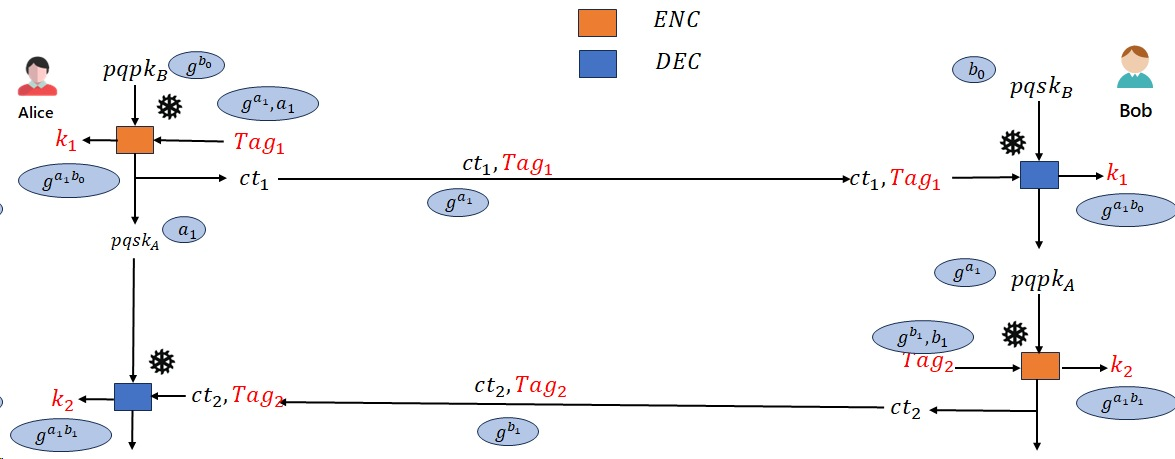
\includegraphics[width=\linewidth]{Img/lc.png} 
    \caption{协议运行的总体流程}
    \label{fig:perf-comparison}
  
  \label{fig:performance}
\end{figure}


\section{方案安全模型}

我们提出一种多阶段认证密钥交换（AKE）协议的安全模型。这个安全模型基于Cohn–Gordon等\cite{cohn2016post}开发的用于分析Signal协议的安全模型改编得到，是一种Bellare – Rogaway式的AKE安全模型\cite{bellare1993entity}。
Bellare–Rogaway式的 AKE 安全模型的基本思想是假定攻击者能够完全掌控协议参与者间的通信，实施如中间人攻击、消息篡改等主动攻击行为，并可通过查询操作泄露长期身份密钥、临时密钥、会话中间状态（随机数、tag）及已建立的会话密钥等各类关键信息。该模型的核心安全性目标是密钥不可区分性，即让攻击者针对选定的目标会话，判断其密钥是协议真实生成的还是等长随机比特串，若攻击者猜测正确概率与随机猜测（1/2）相近，则表明会话密钥对攻击者而言具备随机性，达到安全要求。同时，为应对攻击者可获取大量信息的情况，模型引入新鲜度条件，仅对攻击者未掌握全部密钥输入的 新鲜会话定义安全性。
接下去，我们将从Cohn–Gordon等开发的用于分析Signal协议的安全模型出发，自定义一个AKE安全模型来分析基于TagKEM的端到端加密通信协议的安全性。














\newcommand{\kw}[1]{\textbf{#1}}
\newcommand{\assign}{\leftarrow}
\newcommand{\randassign}{\gets_{\$}}

\begin{definition}{多阶段会话密钥不可区分性（ms-Ind）}
% \label{exp:ki}
我们考虑多阶段密钥交换协议 $\Pi$ 的会话密钥不可区分性（KI）安全属性，形式化定义为安全实验 $\mathsf{Exp}_{\Pi}^{\mathsf{ms-Ind}}(\mathcal{A})$，实验如\ref{fig:security-experiment}所示，由攻击者 $\mathcal{A}$ 参与执行。实验流程如下：
%%%%%%%%%%%%%%%%%%%%%%%%%%%%%%%%%%%%%%
\begin{figure}[htbp]
    \centering
    \caption{Security experiment for adversary $\mathcal{A}$ against multi-stage key indistinguishability of protocol $\Pi$}
    \label{fig:security-experiment}
    \footnotesize

    % 自定义命令：算法标题带下划线
    \newcommand{\algtitle}[1]{%
        \settowidth{\tmpwd}{\textbf{#1}}%
        \textbf{#1}\\[-2pt]%
        \rule{\tmpwd}{0.4pt}%
        \vspace{1mm}%
    }
    \newlength{\tmpwd}

    \begin{minipage}[t]{0.48\textwidth}
        \hrule height 0.8pt
        \vspace{1mm}
        \algtitle{$\mathsf{IND}_{\Pi,n_P,n_B,n_S,n_s}^{\mathcal{A}}$}

        $b \gets_{\$} \{0,1\}$ \\
        $\mathsf{tested} \gets \bot$ \\
        \textbf{for} $P = 1 \dots n_P$ \textbf{do} \\
        \hspace{4mm} $(\mathsf{idecvk}_P, \mathsf{idecsk}_P) \gets_{\$} \mathsf{IDKeyGen}()$ \\
        \hspace{4mm} \textbf{for} $i = 1 \dots n_B$ \textbf{do} \\
        \hspace{8mm} $(\mathsf{preecpk}_{P,i}, \mathsf{preecsk}_{P,i}, \mathsf{prepqpk}_{P,i}, \mathsf{prepqsk}_{P,i}, \sigma) \gets_{\$} \mathsf{PKBGen}(\mathsf{idecsk}_P)$ \\
        \hspace{4mm} \textbf{end for} \\
        \textbf{end for} \\
        $\mathit{pubinfo} \gets (\mathsf{idecvk}_*, \mathsf{preecpk}_*, \mathsf{prepqpk}_*, \sigma_*)$ \\
        $b' \gets \mathcal{A}^{\mathsf{Send},\mathsf{Rev*},\mathsf{Test}}(\mathit{pubinfo})$ \\
        \textbf{if} $(\mathsf{tested} = \bot) \lor \neg \mathsf{fresh}(\mathsf{tested})$ \textbf{then} \\
        \hspace{4mm} $r \gets_{\$} \{0,1\}$ \textbf{ return} $r$ \\
        \textbf{end if} \\
        \textbf{if} $b = b'$ \textbf{then return} $1$ \textbf{ else return} $0$ \textbf{ end if}

        \vspace{3mm}
        \hrule height 0.8pt
        \vspace{1mm}
        \algtitle{$\mathsf{Send}(P,p,m)$}

        \textbf{if} $\pi_{P,p} = \bot$ \textbf{then} \\
        \hspace{4mm} \textbf{parse} $(P', i, \mathsf{role}, m') \gets m$ \\
        \hspace{4mm} \textbf{if} $\mathsf{role} = \mathsf{init}$ \textbf{then return} $\mathsf{SessionStartS}(\pi_{P,p}, \mathsf{idecvk}_{P'}, \mathsf{PKB}_{P',i})$ \\
        \hspace{4mm} \textbf{else if} $\mathsf{role} = \mathsf{resp}$ \textbf{then return} $\mathsf{SessionStartR}(\pi_{P,p}, \mathsf{idecvk}_{P'}, \mathsf{PKB}_{P,i}, m')$ \\
        \hspace{4mm} \textbf{end if} \\
        \textbf{else} \\
        \hspace{4mm} \textbf{parse} $(\mathit{type}, m') \gets m$ \\
        \hspace{4mm} \textbf{if} $\mathit{type} = \mathit{asym}$ \textbf{then return} $\mathsf{AsymRatchet}(\pi_{P,p}, m')$ \\
        \hspace{4mm} \textbf{else} \\
        \hspace{8mm} $\mathit{type} = \mathit{sym}$ \\
        \hspace{8mm} \textbf{parse} $(\mathit{chain}, j) \gets m'$ \\
        \hspace{8mm} \textbf{return} $\mathsf{SymRatchet}(\pi_{P,p}.\mathit{chain}[j])$ \\
        \hspace{4mm} \textbf{end if} \\
        \textbf{end if}
    \end{minipage}
    \hfill
    \begin{minipage}[t]{0.48\textwidth}
        \hrule height 0.8pt
        \vspace{1mm}
        \algtitle{$\mathsf{RevLongTermKey}(P)$}

        $\mathsf{rev\_ltk}[P] \gets \mathsf{true}$ \textbf{ return} $\mathsf{idecsk}_P$

        \vspace{3mm}
        \hrule height 0.8pt
        \vspace{1mm}
        \algtitle{$\mathsf{RevPreKey}(P,i,t)$}

        $\mathsf{rev\_prekey}[P,i,t] \gets \mathsf{true}$ \\
        \textbf{if} $t = \mathsf{ec}$ \textbf{then return} $\mathsf{preecsk}_{P,i}$ \\
        \textbf{else if} $t = \mathsf{pqsk}$ \textbf{then return} $\mathsf{prepqsk}_{P,i}$ \\
        \textbf{else if} $t = \mathsf{pqrnd}$ \textbf{then return} $\mathsf{prepqrnd}_{P,i}$ \\
        \textbf{end if}

        \vspace{3mm}
        \hrule height 0.8pt
        \vspace{1mm}
        \algtitle{$\mathsf{RevRchKey}(P,p,s,t)$}

        $\mathsf{rev\_rchkey}[P,p,s,t] \gets \mathsf{true}$ \\
        \textbf{if} $t = \mathsf{ec}$ \textbf{then return} $\mathsf{rhecsk}_{P,p,s}$ \\
        \textbf{else if} $t = \mathsf{pqsk}$ \textbf{then return} $\mathsf{rchpqsk}_{P,p,s}$ \\
        \textbf{else if} $t = \mathsf{pqrnd}$ \textbf{then return} $\mathsf{rchpqrnd}_{P,p,s}$ \\
        \textbf{end if}

        \vspace{3mm}
        \hrule height 0.8pt
        \vspace{1mm}
        \algtitle{$\mathsf{RevSessKey}(P,p,s)$}

        $\mathsf{rev\_session}[P,p,s] \gets \mathsf{true}$ \textbf{ return} $\pi_{P,p}.k[s]$ as per Table~3

        \vspace{3mm}
        \hrule height 0.8pt
        \vspace{1mm}
        \algtitle{$\mathsf{RevState}(P,p,s)$}

        $\mathsf{rev\_state}[P,p,s] \gets \mathsf{true}$ \textbf{ return} $\pi_{P,p}.st[s]$ \\
        and input intermediate keys in Table~2

        \vspace{3mm}
        \hrule height 0.8pt
        \vspace{1mm}
        \algtitle{$\mathsf{Test}(P,p,s)$}

        \textbf{if} $\mathsf{tested} \neq \bot$ \textbf{then return} $\bot$ \textbf{ end if} \\
        \textbf{if} $\pi_{P,p}.\mathsf{status}[s] \neq \mathsf{accept}$ \textbf{then return} $\bot$ \textbf{ end if} \\
        \textbf{if} $\pi_{P,p}.k[s] = \bot$ \textbf{then return} $\bot$ \textbf{ end if} \\
        $\mathsf{tested} \gets (P,p,s)$ \\
        \textbf{if} $b = 0$ \textbf{then} $k \gets \pi_{P,p}.k[s]$ \textbf{ else} $k \gets_{\$} \mathcal{K}$ \textbf{ end if} \\
        \textbf{return} $k$
    \end{minipage}
\end{figure}
%%%%%%%%%%%%%%%%%%%%%%%%%%%%
\begin{enumerate}[leftmargin=*,noitemsep]
  \item \textbf{实验初始化}：
    \begin{itemize}[leftmargin=*,noitemsep]
      \item 随机选择挑战比特 $b_{\mathsf{test}} \xleftarrow{\$} \{0,1\}$。
      \item 为所有 $n_p$ 个诚实参与方生成长期密钥对：
        \[
        (IPK_P, ISK_P) \leftarrow \mathsf{KeyGen}(), \quad \forall P \in [n_p]
        \]
      \item 向攻击者 $\mathcal{A}$ 提供所有诚实方的长期公钥 $IPK_P$ 和中期公钥 $SPK_P$。
    \end{itemize}

  \item \textbf{攻击者 $\mathcal{A}$ 的自适应查询}：
    攻击者可自适应地发起以下预言机查询：
    \begin{itemize}[leftmargin=*,itemsep=1.2ex]
      \item {$\mathsf{Send}(P, i, m)$}: 向会话 $\pi_P^i$ 发送消息 $m$，并接收其响应。
      
      \item {$\mathsf{CorruptLTKey}(P)$}: 腐败用户 $P$ 的长期身份私钥 $ISK_P$，标记 $\mathsf{corrltk}_P = \mathsf{true}$。
      
      \item {$\mathsf{CorruptSSKey}(P)$}: 腐败用户 $P$ 的中期椭圆曲线私钥 $SSsk_P$，标记 $\mathsf{corrsssk}_P = \mathsf{true}$。
      
      \item {$\mathsf{RevealSessKey}(\pi_P^i, s)$}: 返回会话 $\pi_P^i$ 在阶段 $s$ 的会话密钥 $K[s]$，标记 $\mathsf{revsk}_{\pi_P^i,s} = \mathsf{true}$。
      
      \item {$\mathsf{RevealRchKey}(\pi_P^i, s)$}: 返回会话 $\pi_P^i$ 在阶段 $s$ 的随机数 $\mathsf{rnd}[s]$，标记 $\mathsf{revrnd}_{\pi_P^i,s} = \mathsf{true}$。
      
      \item {$\mathsf{RevealState}(\pi_P^i, s)$}: 返回会话 $\pi_P^i$ 在阶段 $s$ 的完整状态 $\mathsf{st}[s]$，标记 $\mathsf{revstate}_{\pi_P^i,s} = \mathsf{true}$。
      
      \item {$\mathsf{Test}(\pi^*)$}: 
        \begin{itemize}[topsep=0.5ex,itemsep=0.3ex]
          \item 若 $\pi^*$ 是新鲜的（fresh），则返回：
            \[
            \begin{cases}
              \pi^*.K & \text{若 } b_{\mathsf{test}} = 0 \\
              k \xleftarrow{\$} \mathcal{K}_{\mathsf{KE}} & \text{若 } b_{\mathsf{test}} = 1
            \end{cases}
            \]
          \item 否则返回 $\bot$。
        \end{itemize}
    \end{itemize}

  \item \textbf{实验结束}：攻击者 $\mathcal{A}$ 输出猜测比特 $b' \in \{0,1\}$。

  \item \textbf{实验输出}：
    \begin{itemize}[leftmargin=*,noitemsep]
      \item 若 $\pi^*$ 是新鲜的且 $b' = b_{\mathsf{test}}$，则输出 $1$；
      \item 若 $\pi^*$ 是新鲜的且 $b' \neq b_{\mathsf{test}}$，则输出 $0$；
      \item 若 $\pi^*$ 不新鲜，则输出 $b'' \xleftarrow{\$} \{0,1\}$（即随机比特）。
    \end{itemize}
\end{enumerate}

攻击者 $\mathcal{A}$ 在实验中的优势定义为：
\[
\mathbf{Adv}_{\Pi}^{\mathsf{ms}}(\mathcal{A}) = \left| \Pr\left[ \mathsf{Exp}_{\Pi}^{\mathsf{ms}}(\mathcal{A}) = 1 \right] - \frac{1}{2} \right|
\]

\end{definition}

为了捕获以上模型的各阶段参数，定义了协议中的各种输入输出参数，如表\ref{tab:stage_io_combined} 所示：


\begin{table}[htbp]
\centering
\caption{各阶段输入输出参数}
\label{tab:stage_io_combined}
\small % 缩小字体
\setlength{\tabcolsep}{4pt} % 减小列间距
\renewcommand{\arraystretch}{1.3} % 行高微调
\begin{tabular}{@{}llllll@{}}
\toprule
\textbf{Role} & \textbf{Stage} & \textbf{Input State} & \textbf{Input IK} & \textbf{Output State} & \textbf{Output IK} \\
\midrule

init & asym$_0$ 
     & — 
     & — 
     & $ \mathsf{esk}_{(P,1)} $ 
     & $ \pi_P^i.rk[\text{asym}_0],\, \pi_P^i.ck[\text{out}_{0,0}] $ \\
\addlinespace

resp & \makecell[l]{asym$_0$ (in) \\ \& asym$_1$} 
     & — 
     & — 
     & $ \mathsf{esk}_{(P,2)} $ 
     & \makecell[l]{$ \pi_P^i.rk[\text{asym}_0],\, \pi_P^i.ck[\text{in}_{0,0}], $ \\ $ \pi_P^i.rk[\text{asym}_1],\, \pi_P^i.ck[\text{out}_{1,0}] $} \\
\addlinespace

init & \makecell[l]{asym$_j$ (in) \& asym$_{j+1}$,\\ $j \geq 1$, odd} 
     & $ \mathsf{esk}_{(P,j)} $ 
     & $ \pi_P^i.rk[\text{asym}_{j-1}] $ 
     & $ \mathsf{esk}_{(P,j+2)} $ 
     & \makecell[l]{$ \pi_P^i.rk[\text{asym}_j],\, \pi_P^i.ck[\text{in}_{j,0}], $ \\ $ \pi_P^i.rk[\text{asym}_{j+1}],\, \pi_P^i.ck[\text{out}_{j+1,0}] $} \\
\addlinespace

resp & \makecell[l]{asym$_j$ (out) \& asym$_{j+1}$,\\ $j \geq 2$, odd} 
     & $ \mathsf{esk}_{(P,j)} $ 
     & $ \pi_P^i.rk[\text{asym}_{j-1}] $ 
     & $ \mathsf{esk}_{(P,j+2)} $ 
     & \makecell[l]{$ \pi_P^i.rk[\text{asym}_j],\, \pi_P^i.ck[\text{in}_{j,0}], $ \\ $ \pi_P^i.rk[\text{asym}_{j+1}],\, \pi_P^i.ck[\text{out}_{j+1,0}] $} \\
\addlinespace

     & \makecell[l]{sym$_{j,l}$ (in)} 
     & — 
     & $ \pi_P^i.ck[\text{in}_{j,l}] $ 
     & — 
     & $ \pi_P^i.ck[\text{in}_{j,l+1}] $ \\
\addlinespace

     & \makecell[l]{sym$_{j,l}$ (out)} 
     & — 
     & $ \pi_P^i.ck[\text{out}_{j+1,l}] $ 
     & — 
     & $ \pi_P^i.ck[\text{out}_{j,l+1}] $ \\
\bottomrule
\end{tabular}

\medskip
\footnotesize
\textbf{注：} 
\texttt{esk}：临时私钥（ephemeral secret key）；
\texttt{rk}：根密钥（root key）；
\texttt{ck}：链密钥（chain key）；
IK = Intermediate Key（中间密钥）；
“—” 表示无输入或输出。
\end{table}





\begin{definition}[新鲜度]
\label{def:freshness}
在本协议中，新鲜度（freshness）是判断某会话阶段 $s$ 的会话密钥 $K[s]$ 是否可用于 $\mathsf{Test}$ 查询的条件。只有当该阶段密钥是“新鲜的”，攻击者才能在 $\mathsf{ms\text{-}ind}$ 安全实验中对其发起测试。

一个会话阶段 $s$ 的密钥 $K[s]$ 被称为 新鲜的，当且仅当满足以下三个条件：
\begin{enumerate}[label=(\arabic*), wide, labelwidth=!, labelindent=0pt]
  \item \textbf{有效性（ 见定义~\ref{def:valid}）}：  
        该阶段必须已达到 $\mathsf{accepted}$ 状态，且在该阶段被接受之前，攻击者未腐败对端的长期身份密钥 $ISK$。  
        否则，攻击者可通过身份伪造轻易破坏协议安全性。

  \item \textbf{输入未完全泄露（见定义~\ref{def:state_fresh}）}：  
        该阶段用于派生会话密钥的输入参数中，至少有一个未被泄露。  
        由于不同阶段类型（初始密钥建立、非对称棘轮、对称棘轮）的输入不同，该条件根据阶段类型 $t[s]$ 进行定制，如表~\ref{tab:unrev_by_stage} 所示。  
        该定义依赖于以下中间定义：
        \begin{itemize}
          \item 中间会话状态是否被泄露（见定义~\ref{def:input_fresh}）；
          \item 对端在该阶段的输入是否被泄露（见定义~\ref{def:peer_ratchet}）。
        \end{itemize}

  \item \textbf{会话密钥未泄露}：  
        该阶段的会话密钥 $K[s]$ 未通过 $\mathsf{RevealSessKey}$ 查询被泄露，且若存在匹配会话，其对端的对应密钥也未被泄露。
\end{enumerate}
\end{definition}
    
\begin{definition}[有效性]
\label{def:valid}
有效性捕获了一个会话阶段被认为是新鲜的最基本条件：该阶段必须已成功接受，且在该阶段被接受之前，攻击者未获取对端的长期身份密钥（否则可进行身份伪造攻击）。此外，该条件确保即使长期密钥后续被泄露，历史会话仍具有前向安全性。

形式化地，会话 $\pi_P^i$ 在阶段 $s$ 是有效的，当且仅当：
\[
\mathsf{valid}(\pi_P^i, s) = \big( \pi_P^i.\mathsf{status\_exec}[s] = \mathsf{accepted} \big)
\]
\end{definition}

\begin{definition}[对端棘轮新鲜度 ]
\label{def:peer_ratchet}
令 $\mathsf{unrev\_peer}(\pi_P^i, j)$ 表示在会话 $\pi_P^i$ 中，对端在第 $j$ 个非对称棘轮阶段的随机输入未被泄露。即：所有与 $\pi_P^i$ 共享第 $j$ 个非对称棘轮会话标识符的对端会话 $\pi_{\mathsf{pid}}^{p'}$，其阶段 $j$ 的随机数 $\mathsf{rnd}[j]$ 均未被 $\mathsf{RevealRchKey}$ 查询泄露。

形式化定义为：
\[
\begin{aligned}
\mathsf{unrev\_peer}(\pi_P^i, j) = 
  &\ \forall p' : \pi_P^i.\mathsf{sid}[\mathsf{asym}_j] = \pi_{\pi_P^i.\mathsf{pid}}^{p'}.\mathsf{sid}[\mathsf{asym}_j] \\
  &\ \implies \neg \mathsf{revrnd}\big[\pi_{\pi_P^i.\mathsf{pid}}^{p'}, j\big]
\end{aligned}
\]
其中：
\begin{itemize}
  \item $\pi_P^i.\mathsf{pid}$ 是当前会话的对端 ID；
  \item $\pi_{\pi_P^i.\mathsf{pid}}^{p'}$ 表示对端参与方的第 $p'$ 个会话；
  \item $\mathsf{sid}[\mathsf{asym}_j]$ 表示第 $j$ 个非对称棘轮阶段的会话标识符；
  \item $\mathsf{revrnd}[\cdot, j]$ 标记该阶段的随机数是否已被泄露。
\end{itemize}
\end{definition}

\begin{definition}[状态新鲜度]
\label{def:state_fresh}
令 $\mathsf{unrev\_state}(\pi_P^i, s)$ 表示会话 $\pi_P^i$ 在阶段 $s$ 的中间状态未被泄露，且其所有匹配的对端会话的对应阶段状态也未被泄露。形式化定义为：
\[
\begin{aligned}
\mathsf{unrev\_state}(\pi_P^i, s) = 
  &\ \neg \mathsf{revstate}[\pi_P^i, s] \\
  &\ \land \left( \forall p' : \pi_P^i.\mathsf{sid}[s] = \pi_{\pi_P^i.\mathsf{pid}}^{p'}.\mathsf{sid}[s] \right. \\
  &\ \left. \implies \neg \mathsf{revstate}\big[\pi_{\pi_P^i.\mathsf{pid}}^{p'}, s\big] \right)
\end{aligned}
\]
其中：
\begin{itemize}
  \item $\mathsf{revstate}[\pi_P^i, s]$ 表示 $\mathsf{RevealState}(\pi_P^i, s)$ 是否已被调用；
  \item 匹配会话通过 $\mathsf{sid}[s]$ 相等来识别；
  \item 该定义确保双方向的状态均未泄露，防止攻击者通过状态泄露重构密钥。
\end{itemize}
\end{definition}

\begin{definition}[阶段更新输入新鲜度]
\label{def:input_fresh}
 $\mathsf{unrev}(\pi_P^i, s)$ 表示会话 $\pi_P^i$ 在阶段 $s$ 的密钥导出输入中，至少有一个未被泄露。由于不同阶段类型的密钥派生依赖不同的输入参数，该条件按阶段类型 $t[s]$ 分别定义如表2所示：



 


% //////////////
\begin{table}[htbp]
\centering
\caption{阶段更新输入新鲜度 $\mathsf{unrev}(\pi_P^i, s)$ 的分阶段定义}
\label{tab:unrev_by_stage}
\small
\setlength{\tabcolsep}{5pt}
\renewcommand{\arraystretch}{1.4}
\begin{tabular}{@{}lll@{}}
\toprule
\textbf{Stage} & \textbf{Role} & \textbf{$\mathsf{unrev}(\pi_P^i, s)$} \\
\midrule

Session init & init & 
$\neg \mathsf{corrsssk}_R \land \neg \mathsf{corrltk}_R \land \neg \mathsf{revrnd}[P,0]$ \\

Session init & resp & 
$\neg \mathsf{corrltk}_P \land \mathsf{unrev\_peer}(P, 1)$ \\

Asym$[j]$, $j>0$, odd & init & 
$\begin{aligned}
&\big( \mathsf{unrev\_state}(\pi_P^i, \mathrm{asym}[j]) \land \mathsf{unrev}(\pi_P^i, \mathrm{asym}[j-1]) \big) \\
\lor\ &\big( \neg \mathsf{revrnd}[\pi_P^i, j] \land \mathsf{unrev\_peer}(\pi_P^i, j+1) \big)
\end{aligned}$ \\

asym$[j+1]$, $j>0$, odd & init & 
$\begin{aligned}
&\big( \mathsf{unrev\_state}(\pi_P^i, \mathrm{asym}[j+1]) \land \mathsf{unrev}(\pi_P^i, \mathrm{asym}[j]) \big) \\
\lor\ &\big( \neg \mathsf{revrnd}[\pi_P^i, j+2] \land \mathsf{unrev\_peer}(\pi_P^i, j+1) \big)
\end{aligned}$ \\

asym$[j]$, $j>0$, odd & resp & 
same as for $\mathrm{asym}[j]$, $j>0$, odd with role = init \\

asym$[j+1]$, $j>0$, odd & resp & 
same as for $\mathrm{asym}[j+1]$, $j>0$, odd with role = init \\

sym$[j,0]$ & any & 
$\mathsf{unrev\_state}(\pi_P^i, \mathrm{sym}[j,0]) \land \mathsf{unrev}(\pi_P^i, \mathrm{asym}[j])$ \\

sym$[j,l]$ & any & 
$\mathsf{unrev\_state}(\pi_P^i, \mathrm{sym}[j,l]) \land \mathsf{unrev}(\pi_P^i, \mathrm{sym}[j-1])$ \\ 
\bottomrule
\end{tabular}

\medskip
\footnotesize
\textbf{注：}
- $\mathsf{corrltk}_X$: 参与方 $X$ 的长期身份密钥被腐败；
- $\mathsf{corrsssk}_X$: 参与方 $X$ 的中期签名密钥被腐败；
- $\mathsf{revrnd}[P]$: 初始随机输入被泄露；
- $\mathsf{unrev\_peer}(P,j)$: 定义见 \ref{def:peer_ratchet}，表示对端第 $j$ 个棘轮输入未泄露；
- $\mathsf{unrev\_state}$: 定义见 \ref{def:state_fresh}；
- “same as” 表示复用对应角色下的相同逻辑，避免重复。
\end{table}

% ？？




\end{definition}


综上，新鲜度捕获了会话密钥合理安全所必需的一切：阶段是有效的，相关中间输入值是不能泄露的，敌手在任何匹配的会话中都没有泄露该阶段或该阶段对端的会话密钥。形式化定义如下所示：
\[
\begin{aligned}
\mathsf{fresh}(\pi_P^i, s) = 
  &\ \mathsf{valid}(\pi_P^i, s) \\
  &\ \land \mathsf{unrev}(\pi_P^i, s) \\
  &\ \land \neg \pi_P^i.\mathsf{revsk}[s] \\
  &\ \land \left( \forall j : \pi_P^i.\mathsf{sid}[s] = 
     \pi_{\pi_P^i.\mathsf{pid}}^j.\mathsf{sid}[s] \Rightarrow 
     \neg \pi_{\pi_P^i.\mathsf{pid}}^j.\mathsf{revsk}[s] \right)
\end{aligned}
\]

%%%%%%%%%%%%%%%%%%%%%%%%%%%%%%%%%
\section{方案安全分析}


\begin{theorem}[会话密钥的安全性 (Key Indistinguishability)]\label{thm:key-indist}
若签名算法满足强不可伪造性（$\mathsf{EUF\text{-}CMA}$），$\mathsf{TKEM}$ 满足 $\mathsf{IND\text{-}CCA2}$ 安全性，$\mathsf{ECDH}$ 满足 $\mathsf{PRF\text{-}ODH}$ 假设，且哈希函数 $H$ 在随机预言机模型（$\mathsf{ROM}$）下，则对于任何新鲜阶段 $s$，对手 $\mathcal{A}$ 在区分会话密钥 $\mathsf{ms\_sk}_s$ 实验中的优势是可忽略的，即：
\begin{equation}
    \mathsf{Adv}_{\Pi}^{\mathsf{ms\text{-}ind}}(\mathcal{A}) \leq \mathsf{Adv}_{\mathsf{Sig}}^{\mathsf{EUF\text{-}CMA}}(\mathcal{B}_1) + \mathsf{Adv}_{\mathsf{TagKEM}}^{\mathsf{IND\text{-}CCA2}}(\mathcal{B}_2) + \mathsf{Adv}_{\mathsf{ECDH}}^{\mathsf{PRF\text{-}ODH}}(\mathcal{B}_3) + \mathsf{Adv}_{H}^{\mathsf{ROM}}(\mathcal{B}_4)
\end{equation}
\end{theorem}

\begin{proof}
我们采用博弈序列（Game-hopping）方法进行证明。定义 $\mathsf{Game}_i$ 为第 $i$ 个博弈，$\Pr[\mathsf{Game}_i]$ 表示对手在该博弈中成功的概率。

\paragraph{$\mathsf{Game}_0$: 原始安全实验}
这是攻击者 $\mathcal{A}$ 与仿真器之间进行的标准 $\mathsf{MS\text{-}AKE}$ 实验。根据定义：
\begin{equation}
    \mathsf{Adv}_{\Pi}^{\mathsf{ms\text{-}ind}}(\mathcal{A}) = \left| \Pr[\mathsf{Game}_0] - \frac{1}{2} \right|
\end{equation}

\paragraph{$\mathsf{Game}_1$: 认证失败情况 (Identity Forgery)}
在此博弈中，如果对手 $\mathcal{A}$ 在未执行 $\mathsf{CorruptLTKey}(P)$ 之前，伪造了一个有效的长期签名或预签名，则游戏终止并输出随机比特。

\textbf{归约：} 若 $\mathcal{A}$ 能成功伪造，则可以构造一个算法 $\mathcal{B}_1$ 攻破签名算法的 $\mathsf{EUF\text{-}CMA}$ 安全性。

\textbf{结果：} 在 $\mathsf{Game}_1$ 之后，我们可以假设所有接收到的协议消息确实是由声称的发送方生成的。因此：
\begin{equation}
    \left| \Pr[\mathsf{Game}_1] - \Pr[\mathsf{Game}_0] \right| \leq \mathsf{Adv}_{\mathsf{Sig}}^{\mathsf{EUF\text{-}CMA}}(\mathcal{B}_1)
\end{equation}

\paragraph{$\mathsf{Game}_2$: 初始密钥交换阶段 (Initial Stage)}
针对阶段 $s=1$（Initial Key Exchange），会话密钥由 $\mathsf{KDF}(rk_0, \mathsf{ecss}, \mathsf{pqss}, \tau)$ 派生。根据新鲜度定义，至少 $\mathsf{ecss}$ 或 $\mathsf{pqss}$ 之一未泄露。

\begin{itemize}[leftmargin=*]
    \item[\textbf{Case 2.1 (经典安全):}] 假设对手是经典的，即便 $\mathsf{PQ}$ 密钥泄露。安全性归约至 $\mathsf{ECDH}$ 的 $\mathsf{PRF\text{-}ODH}$ 假设。
    
    \item[\textbf{Case 2.2 (抗量子安全):}] 假设对手拥有量子能力。此时安全性归约至 $\mathsf{TagKEM}$ 的 $\mathsf{IND\text{-}CCA2}$ 安全性。即使对手拥有 $\mathsf{sk}_{\mathsf{pq}}$，但由于 $\mathsf{ss} = \mathsf{Decaps}(\mathsf{sk}_{\mathsf{pq}}, c, \tau)$，且 $\tau$ 包含了新鲜的临时 $\mathsf{DH}$ 信息，对手无法计算出 $\mathsf{pqss}$。
\end{itemize}

因此：
\begin{equation}
    \left| \Pr[\mathsf{Game}_2] - \Pr[\mathsf{Game}_1] \right| \leq \mathsf{Adv}_{\mathsf{TagKEM}}^{\mathsf{IND\text{-}CCA2}}(\mathcal{A}) + \mathsf{Adv}_{\mathsf{ECDH}}^{\mathsf{PRF\text{-}ODH}}(\mathcal{A})
\end{equation}

\paragraph{$\mathsf{Game}_3$: 非对称棘轮阶段 (Asymmetric Ratchet)}
这是证明的核心。每一轮非对称棘轮都会引入新的 $\mathsf{ecss}$ 和通过 $\mathsf{TagKEM}$ 生成的 $\mathsf{pqss}$。

\textbf{后攻破安全性 (PCS) 的论证：} 假设对手在阶段 $s-1$ 执行了 $\mathsf{CorruptSSKey}$ 获取了当前状态。在阶段 $s$ 中，诚实参与者交换了新的临时 $\mathsf{EC}$ 公钥，并生成了新的标签 $\tau_s$。根据 $\mathsf{TagKEM}$ 的 $\mathsf{IND\text{-}CCA2}$ 性质，由于 $\tau_s$ 是新鲜且未被篡改的，即便对手知道之前的状态，在没有当前阶段新鲜 $\mathsf{DH}$ 贡献的情况下，他也无法计算出新的根密钥 $rk_s$。

\textbf{结论：} 每一轮非对称棘轮都重新确立了安全性屏障。

\paragraph{$\mathsf{Game}_4$: 对称棘轮阶段 (Symmetric Ratchet)}
对称棘轮仅通过单向函数（如 $\mathsf{HMAC}$ 或 $H$）演进链密钥 $\mathsf{ck}$。

\textbf{归约：} 安全性归约至哈希函数的抗原像性或 $\mathsf{PRG}$（伪随机生成器）属性。

\textbf{结果：} 保证了消息密钥 $\mathsf{mk}$ 的前向安全性（Forward Secrecy）。

\paragraph{最终优势界限}
综合上述所有博弈，我们得到：
\begin{align}
    \mathsf{Adv}_{\Pi}^{\mathsf{ms\text{-}ind}}(\mathcal{A}) &= \left| \Pr[\mathsf{Game}_4] - \frac{1}{2} \right| \nonumber \\
    &\leq \sum_{i=1}^{4} \left| \Pr[\mathsf{Game}_i] - \Pr[\mathsf{Game}_{i-1}] \right| \nonumber \\
    &\leq \mathsf{Adv}_{\mathsf{Sig}}^{\mathsf{EUF\text{-}CMA}}(\mathcal{B}_1) + \mathsf{Adv}_{\mathsf{TagKEM}}^{\mathsf{IND\text{-}CCA2}}(\mathcal{B}_2) \nonumber \\
    &\quad + \mathsf{Adv}_{\mathsf{ECDH}}^{\mathsf{PRF\text{-}ODH}}(\mathsf{B}_3) + \mathsf{Adv}_{H}^{\mathsf{ROM}}(\mathcal{B}_4)
\end{align}

由于所有底层原语的优势均为可忽略函数，故 $\mathsf{Adv}_{\Pi}^{\mathsf{ms\text{-}ind}}(\mathcal{A})$ 也是可忽略的。
\end{proof}